\chapter{Design of MPI\_T support in CALIPER}

Caliper is an application introspection tool that relies on source code annotations to collect information and perform profiling related tasks. I shall first provide a basic overview of relevant Caliper concepts before describing the MPI\_T support in Caliper. 

\section{Caliper Concepts}
\subsection{Caliper API}
Caliper provides an application level API that acts as the portal for carrying out performance measurements. Caliper also provides high-level annotation macros that are user-friendly. The basic idea behind the source-code annotation API is to associate performance measurements with user-defined, high-level \textit{context information}. These source code annotations act as hooks for background processing. Caliper is built into a library and linked into the application. Figure \ref{fig:caliexample}\footnote{Image taken from: https://llnl.github.io/Caliper} is an example of a Caliper-annotated \verb+C+\texttt{++} source code.
\subsection{Attributes: Caliper's Building Blocks}
Caliper provides a generic \textit{key-value} data model for storing performance data of all kinds. Caliper \textit{attributes} are the basic elements of the Caliper data model. The keys need to have a unique name and a type. They can also optionally have properties which determine how the attributes get processed. An example would be an attribute to track PAPI counters or an attribute to track the total time spent inside a routine or code section. 
\par Among all the properties that an attribute can have, the most important attribute in the context of MPI\_T is the \verb+AS_VALUE+ property. Attributes with the \verb+AS_VALUE+ property set to true cannot be nested. For example, the attribute to track PAPI counters cannot be nested, but the attribute to track the time spent inside a routine is nested.
\begin{center}
	\begin{figure*}[tbp!]
         \centering
		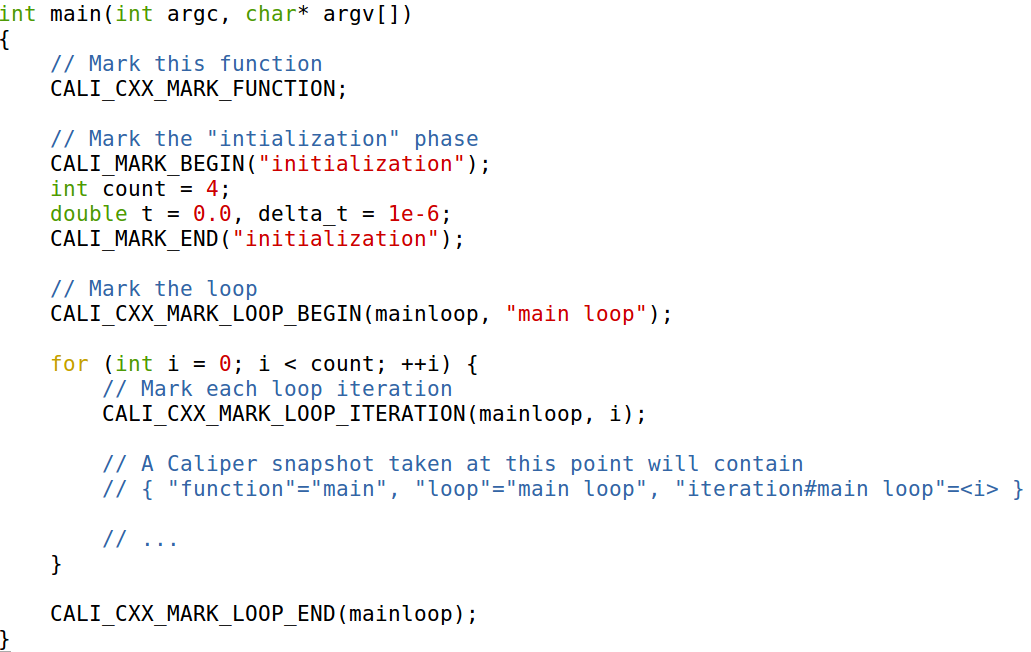
\includegraphics[scale=0.3, width=\columnwidth, keepaspectratio]{figures/cali-example}
		\caption{Caliper~\cite{CALIPER} Annotated Source Code}
		\label{fig:caliexample}
	\end{figure*}
\end{center}

\subsection{Blackboards and Snapshots}
Whenever a performance measurement is made by use of Caliper's measurement API, the values of one or more attributes are updated in an internal data-structure referred to as the \textit{blackboard}. This blackboard is a runtime buffer that is used to combine active attributes, and is updated by Caliper data providers (annotations).
\par A \textit{snapshot} saves the current context of the blackboard. A snapshot can be triggered independently of blackboard updates. Additional information can be added to the snapshot via callbacks to snapshot events. 
\subsection{Services}
Caliper \emph{services} are the basic building blocks that can be combined freely to realize advanced profiling/tracing capabilities. Services are essentially plugins that register callbacks for events of interest. During Caliper initialization, the registered initialization function of each required service is invoked, and the service then performs start-up related tasks inside this initialization function. 
\par An example of a service is the \textit{MPI} service. The MPI service keeps track of the time spent inside MPI calls by utilizing the PMPI interface. The \textit{recorder} service writes Caliper snapshot records into a file using a custom text-based I/O format. The recorder service in conjunction with the MPI service can be used to gather a basic profile of an MPI application. Figure \ref{fig:caliservices} is an illustration of this use case. 
\begin{center}
	\begin{figure*}[bp!]
         \centering
		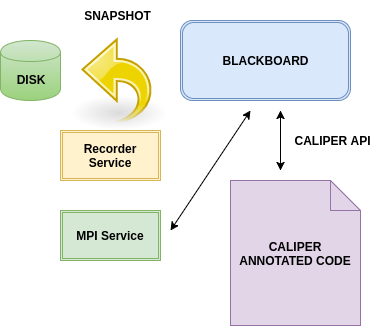
\includegraphics[scale=0.7, keepaspectratio]{figures/cali-services}
		\caption{MPI Profiling: Caliper~\cite{CALIPER} Service Flow}
		\label{fig:caliservices}
	\end{figure*}
\end{center}

\section {MPI\_T Service: Supporting Performance Introspection}
This section describes the design of the MPI\_T service that performs runtime MPI library introspection through the MPI\_T interface. As of the time being, this service does not support performance monitoring or tuning through the MPI\_T interface. 
\section{Service Registration}
During the registration phase for the MPI\_T service, the MPI\_T performance session is created. The handles for all the PVARs exported at the time of service registration are allocated. It is important to note that service registration may happen before \verb+MPI_Init+ is invoked. If this is the case, the number of PVARs exported would be zero. The design should account for this scenario.
\par In the next section, I shall discuss the complexities that arise with allocating handles for PVARs in detail, and how the design addresses these issues.
\section{PVAR Handle Allocation}
Before a tool can read the value of a PVAR, it must first allocate a \emph{handle} for the PVAR. The MPI\_T interface specifies a function that allows a tool to know the number of PVARs exported by an MPI implementation at any given point in time. Recall that the number of PVARs exported can dynamically increase, and that PVARs can be bound to MPI objects. Like TAU, Caliper only supports PVARs that are exported immediately after \verb+MPI_Init+ by invoking the handle allocation routine inside the PMPI wrapper for \verb+MPI_Init+. Any increase in the number of PVARs after this point is ignored by Caliper. 
\par PVARs can be bound to MPI objects, and such PVARs can provide fine-grained detail about MPI. For example, a PVAR representing the number of messages sent can potentially be bound to an MPI communicator object. This way, it would be possible for a tool to distinguish the quantity of communication across communicators/process groups, instead of presenting an aggregated view to the user.
\par Handles for PVARs not bound to any object (\verb+MPI_T_BIND_NO_OBJECT+) can be allocated at any time --- specifically, this is done inside the registration phase for the MPI\_T service, and inside the PMPI wrapper for \verb+MPI_Init+. In order to allocate handles for PVARs bound to MPI objects, we need a reference (address) for the MPI object in question. The ideal location for the MPI\_T service to grab these references would be during MPI object creation. Briefly, the following steps are necessary to allocate such handles:
\begin{itemize}
\item Identify the corresponding MPI object creation routine for the object in question
\item Intercept the object creation routine (through PMPI)
\item Allocate handles for all PVARs bound to the given object type
\end{itemize}
It is possible that multiple handles are associated with PVARs bound to MPI objects. The supported MPI object types in MPI\_T and their corresponding object routines used to allocate handles are presented in Table \ref{tab:caliperhandles}.
\begin{table*}[!htbp]
  \centering
  \small
  \captionsetup{justification=centering}
  \caption{Caliper: PVAR Handle allocation routines for supported MPI object types}
  \label{tab:caliperhandles}
  \resizebox{0.65\columnwidth}{!}{\begin{tabular}{|c|l|}
    \toprule
    MPI Object Type&MPI Object Creation Routine\\
     \midrule
     MPI Communicator&MPI\_Comm\_Create\\
     MPI Error Handler&MPI\_Err\_handler\\
     MPI File&MPI\_File\_open\\
     MPI Groups&MPI\_Group\_create\\
     MPI Reduction Operators&MPI\_Op\_create\\
     MPI Info Objects&MPI\_Info\_create\\
     MPI Window Objects&MPI\_Win\_create\\
     MPI Datatypes&\textit{Not Supported}\\
     MPI Message Objects&\textit{Not Supported}\\
     MPI Request Objects&\textit{Not Supported}\\
  \bottomrule
\end{tabular}}
\end{table*}

\section{PVAR Classes and Notion of Aggregability}
Depending on what they represent, PVARs are categorized by the MPI standard into counters, state variables, watermarks, etc., and are handled differently by Caliper. We define the notion of \textit{aggregatability} as follows: Any PVAR on which it is \emph{meaningful} to apply one or more of the operators --- SUM, MAX, MIN, AVG, COUNT is defined as aggregatable.
\par Along with other information, a call to \verb+MPIT_pvar_get_info+ returns the \emph{CLASS} to which the PVAR belongs. Below we describe the various PVAR classes supported by the MPI standard and how each class is handled by Caliper:
\begin{itemize}
	\item \verb+MPI_T_PVAR_CLASS_TIMER+, \verb+MPI_T_PVAR_CLASS_AGGREGATE+, \verb+MPI_T_PVAR_CLASS_COUNTERS+: These are free-counting, monotonically increasing values. As such, they are not aggregatable, but by storing the previous value for these counters and timers, the difference between the current and previous value is a derived metric that is aggregatable by use of \emph{SUM}, \emph{MAX}, \emph{MIN}, \emph{AVG} operators. Storing this difference is more useful than just the raw counter values, as one would typically be interested in the \emph{change} caused to any of these PVARs rather than the raw value itself.
	\item \verb+MPI_T_PVAR_CLASS_STATE+: Represents MPI state at any instant in time. Non-aggregatable value.
	\item \verb+MPI_T_PVAR_CLASS_SIZE+: Represents size of an MPI resource. Non-aggregatable value.
	\item \verb+MPI_T_PVAR_CLASS_LEVEL+, \verb+MPI_T_PVAR_CLASS_PERCENTAGE+: Represents the instantaneous level or percentage utilization of an MPI resource. It is meaningful to apply the \emph{AVG}, \emph{MIN}, \emph{MAX} operators, and hence these classes are aggregatable.
	\item \verb+MPI_T_PVAR_CLASS_HIGHWATERMARK+, \verb+MPI_T_PVAR_CLASS_LOWWATERMARK+: As such, these classes are non-aggregatable. However, one can define aggregatable derived metrics out of these PVARs. Specifically, Caliper defines two derived metrics --- A boolean that tells us if the watermark has gone up from the last time it was read, and a double value specifying the \emph{change} in the value between successive reads. Both of these derived metrics are aggregatable quantities as one can apply the \emph{COUNT} and/or \emph{SUM} operator to them.
	\item \verb+MPI_T_PVAR_CLASS_GENERIC+: PVARs that do not fall into any of the above classes. These PVARs would need to be handled on a case-by-case basis, and thus, for now, we define these to be non-aggregatable.
\end{itemize}

\section{Creating Caliper Attributes for PVARs}
The basic data unit in Caliper is an attribute. An attribute is a key-value pair that has certain properties. For each PVAR exposed by the MPI library, Caliper defines an attribute with the same name as the PVAR. Each PVAR attribute has the following properties:
\begin{itemize}
	\item \verb+CALI_ATTR_AS_VALUE+ - We do not want "stacking" semantics for PVAR values. They should be treated much the same way as PAPI counters.
	\item \verb+CALI_ATTR_SCOPE_PROCESS+ - PVARs are defined on a per-rank basis
	\item \verb+CALI_ATTR_SKIP_EVENTS+ - We do not want callbacks to be triggered every time the attribute for a PVAR is updated
	\item \verb+Metadata (class.aggregatable)+ - Boolean value specifying if the PVAR is aggregatable or not. Aggregatability is determined based on the class to which a PVAR belongs. 
\end{itemize}
Apart from creating a Caliper attribute for each PVAR exported, two additional attributes are created for each \textit{watermark class} PVAR exported --- one that represents the number of times the watermark changes, and another that represents the cumulative change in the watermark PVAR.

\section{Sampling and Storing PVARs in Snapshots}
All PVARs exported by the MPI library are queried when a snapshot is triggered. For example, when the MPI service is enabled, snapshots are taken every time an MPI call is made. By integrating the MPI\_T service along with the MPI service, we would be able to determine how various MPI function calls contribute to changes in PVAR values. One can gather meaningful information by aggregating PVAR values using MPI function names or annotated code regions as keys --- this would be particularly helpful in attributing MPI inefficiencies down to source code sections or MPI routines. 
\par Depending on the class of the PVAR, we either store the raw value read from the interface in the snapshot, or a derived metric. Below, we describe various PVAR classes are represented in the snapshot:
\begin{itemize}
	\item \verb+MPI_T_PVAR_CLASS_TIMER+, \verb+MPI_T_PVAR_CLASS_AGGREGATE+, \verb+MPI_T_PVAR_CLASS_COUNTERS+: We store the difference between the current value and the previous for such PVARs in the snapshot. Storing and aggregating this derived value is more meaningful than storing the raw value --- it helps us answer questions such as: 
 \begin{itemize}
   \item How do different MPI functions contribute to this PVAR? 
   \item Which MPI function is responsible for the highest value?
 \end{itemize}
	\item \verb+MPI_T_PVAR_CLASS_STATE+, \verb+MPI_T_PVAR_CLASS_SIZE+: The raw values of such PVARs are stored in the snapshot. It may be more meaningful to view changes of these PVARs \emph{over time}, such as in a trace.
	\item \verb+MPI_T_PVAR_CLASS_HIGHWATERMARK+, \verb+MPI_T_PVAR_CLASS_LOWWATERMARK+: Along with storing the raw value for watermark PVARs, we store the derived metrics that represent the number of times the watermark changed, along with how much the watermark changed in the snapshot. By aggregating across MPI functions for example, we can answer questions such as: 
 \begin{itemize}
   \item Which function most frequently pushed up/down a watermark? 
   \item Which function was responsible for the highest cumulative change in a given watermark?
 \end{itemize}
 \item \verb+MPI_T_PVAR_CLASS_LEVEL+, \verb+MPI_T_PVAR_CLASS_PERCENTAGE+: The raw values of such PVARs are stored in the snapshot. It maybe meaningful to view the average, maximum, or minimum value for these PVARs aggregated across MPI functions.
\end{itemize}

\section{Usage Scenarios}
As of the writing of this document, Caliper only supports performance introspection through the MPI\_T interface, so the set of usage scenarios is limited in variety. The design of the performance introspection support in Caliper was carried out with one specific goal --- to analyze PVAR values \textit{across annotated code sections} using the \textit{aggregate service}.
\par In other words, we would like \textit{attribute} changes in PVAR values to specific code regions or function invocations. In this way, we hope that MPI\_T would allow us to narrow down performance inefficiencies to specific locations in the source code. The following two usage scenarios are an attempt to showcase this design.
\subsection{Detecting Performance Inefficiencies in MPI}
With this use case, we would like to answer this specific question --- What are the contributions of different MPI routines to PVARs that represent an \textit{aggregatable} quantity such as memory allocated within MPI?
\par Sampling and storing PVARs is likely to be more effective if the context information is stored along with it for analysis later on. If we are able to identify the contributions of various MPI routines to the final sampled value of a PVAR at the end of a run, this could aid in narrowing down causes for performance inefficiencies \textit{within} the MPI library itself. 
\par As discussed in an earlier section introducing Caliper concepts, \textit{services} act as basic building blocks for realizing more advanced functionality. Below, I briefly discuss the key services that are used to enable such a functionality:
\subsubsection{Event Service}
The event trigger service triggers snapshots when attributes are updated. Recall that whenever a snapshot is triggered, the MPI\_T interface is queried. Through the environment variable \verb+CALI_EVENT_TRIGGER+, the user can specify a list of attributes whose updates triggers a snapshot. Attributes that have the \verb+CALI_ATTR_SKIP_EVENTS+ property set do not trigger snapshots. PVAR attributes have this property set to true.
\subsubsection{MPI Service}
This service records MPI operations and the MPI rank. This service utilizes the PMPI interface to keep a track of the program execution time spent inside MPI. MPI function names are stored in the special attribute \verb+mpi.function+ and the MPI rank in the \verb+mpi.rank+ attribute.
\subsubsection{Aggregate Service}
The aggregate service accumulates aggregation attributes (e.g. time durations) of snapshots with a similar \textit{key}, creating a profile. The environment variable \verb+CALI_AGGREGATE_KEY+ is used to specify the colon-separated list of attributes that for the aggregation key. It is important to note that these attributes can not have the \verb+AS_VALUE+ property set to true. An example of such an attribute would be \verb+mpi.function+ or \verb+mpi.rank+.
\par Through the environment variable \verb+CALI_AGGREGATE_ATTRIBUTES+, the user can specify the list of aggregation attributes. These attributes must have the \verb+AS_VALUE+ property set to true. All PVARs are candidates for such attributes. The aggregate service aggregates values of aggregation attributes from all input snapshots with similar aggregation keys.
\subsubsection{Report Service}
The report service aggregates, formats, and writes collected Caliper records into files or stdout on Caliper flush events (typically, at program end). By default, the report service prints a tabular, human-readable report of the collected snapshots.

\section{Target Applications}
\section{Experiments}

\section {Implementation Challenges and Issues}
\subsection{Crashes with OpenMPI}
The MPI\_T support in Caliper was designed to be specifically used with the OpenMPI implementation. When this research was being carried out, OpenMPI was the only MPI library that had support for PVARs bound to MPI objects. However, we noted that the application crashed when we were trying to allocate handles for PVARs bound to MPI objects. This issue was communicated to the developers of the OpenMPI library. Unfortunately, this issue was not resolved in time, and we had to use MVAPICH2 for testing purposes.

\subsection{Lack of GUI support in Caliper}
When this research was being conducted, Caliper did not have GUI support for visualizing profiles, nor did it have support for writing out traces in a standard format. Caliper had basic text-based support for viewing and analyzing the collected performance data. Given the relatively large number of PVARs exported by MVAPICH2 (~100), the basic text-based support was not sufficient to display all the data. We had to resort to viewing only a subset of PVARs at any given time.
